\documentclass[12pt,a4paper,leqno]{report}

\usepackage[ansinew]{inputenc}
\usepackage[T1]{fontenc}
\usepackage[english]{babel}
\usepackage{amsthm}
\usepackage{amsfonts}         
\usepackage{amsmath}
\usepackage{amssymb}
\usepackage{enumitem}
\usepackage{fixltx2e}
\usepackage{tikz}
\usepackage{mathabx}
\usetikzlibrary{calc}



\newcommand{\argmax}{\operatornamewithlimits{argmax}}
\newcommand{\R}{\mathbb{R}}
\newcommand{\C}{\mathbb{C}}
\newcommand{\Q}{\mathbb{Q}}
\newcommand{\N}{\mathbb{N}}
\newcommand{\No}{\mathbb{N}_0}
\newcommand{\Z}{\mathbb{Z}}
\newcommand{\diam}{\operatorname{diam}}
\newcommand{\ob}{\operatorname{ob}}

\newcommand\opn{\mathrel{\ooalign{$\subset$\cr
			\hidewidth\hbox{$\circ\mkern.5mu$}\cr}}}
\newcommand\cls{\mathrel{\ooalign{$\subset$\cr
			\hidewidth\hbox{$c\mkern.5mu$}\cr}}}
\newcommand*{\QEDA}{\hfill\ensuremath{\blacksquare}}%

\theoremstyle{plain}
\newtheorem{lause}[equation]{Theorem}
\newtheorem{lem}[equation]{Lemma}
\newtheorem{prop}[equation]{Proposition}
\newtheorem{kor}[equation]{Corollary}
\newtheorem{vaite}{V�ite}

\setcounter{secnumdepth}{3}
\newcounter{diagram}
\numberwithin{diagram}{subsection}
\newenvironment{diagram}
{\stepcounter{diagram}\par\smallskip\noindent\begin{minipage}{\linewidth}\centering}
	{\par Diagram~\thediagram\end{minipage}\par\smallskip}
\theoremstyle{definition}
\newtheorem{maar}[equation]{Definition}
\newtheorem{konj}[equation]{Conjecture}
\newtheorem{esim}[equation]{Example}

\theoremstyle{remark}
\newtheorem{huom}[equation]{Huomautus}

\pagestyle{plain}
\setcounter{page}{1}
\addtolength{\hoffset}{-1.15cm}
\addtolength{\textwidth}{2.3cm}
\addtolength{\voffset}{0.45cm}
\addtolength{\textheight}{-0.9cm}


\title{Cech (co)homology}
\author{Yury Elkin}
\date{}



\begin{document}

\maketitle

\tableofcontents

\chapter{Inroduction}\label{johd}



\chapter{Background}

In this chapter we will recall a few details about algebra, category theory and abstract simplicial complexes. We assume that the reader is familiar with basic concepts of homology and cohomology theory and constructions related to them.

\section{Direct sum and direct product}
In this section we will recall a few details about direct sums and direct products.
\begin{maar}
Let $\{A_i\}_{i \in J}$ be a family of groups. The direct product of these groups is the Cartesian product $\prod_{i \in J} A_i$ where addition is defined component-wise $(a+b)_i = a_i+_ib_i$
\end{maar}
\begin{maar}
Let $\{A_i\}_{i \in J}$ be a family of groups. The direct sum of these groups is the subgroup of direct product given by  $\bigoplus_{i \in J}A_i = \{x \in \prod_{i \in J} A_i \mid x_i \neq 0 \text{ for only finetely many } i \}. $
\end{maar}
For direct sums and direct products we have following universal properties:
\begin{lem}\label{Universalpropertyproduct}
Let $A = \prod_{i \in J} A_i$ be the direct sum and $D$ an arbitrary group. Then for every set of homomorphisms $\{f_i:D \rightarrow A_i\}_{i \in J}$ there exists a unique homomorphism $f:D \rightarrow A$ for which condition $pr_i \circ f = f_i $ holds for every $i \in J$.
\end{lem}
\begin{proof}
Proved in [\ref{algebra2}] theorem 3.7.
\end{proof}
\begin{lem}\label{Universalpropertysum}
	Let $A = \bigoplus_{i \in J}A_i$ be the direct sum and $D$ an arbitrary group. Then for every set of homomorphisms $\{f_i:A_i \rightarrow D\}_{i \in J}$ there exists a unique homomorphism $f:A \rightarrow D$ for which the condition $ f \circ j_i = f_i $ holds for every $i \in J$.
\end{lem}
\begin{proof}
Proved in [\ref{algebra2}] theorem 3.6.
\end{proof}
\section{Category theory}

In this thesis we will present theory in a categorical way, which will make the construction more general. First lets recall the definition of a category. 

\begin{maar}
A category C consist of the following ingredients: A class of objects $\ob(C)$, a class of morphisms $\hom(C)$ for which and for every objects $A$, $B$ in $\ob(C)$ there exists a subclass $Hom(A,B)$ and a rule of composition $Comp:Hom(A,B) \times Hom(B,D) \rightarrow Hom(A,D)$ for which following conditions hold:
\begin{enumerate}[label=(\arabic*),ref=(\arabic*)]
	
	
	\item Composition is associative. Let $f:A \rightarrow B$, $g: B \rightarrow D$ and $h: D \rightarrow E$ be morphisms between objects then $(f \circ g) \circ h = f \circ (g \circ h)$
	
	\item For every object $A \in \ob(C)$ there exists identity morphism $1_A \in \hom(A,A)$ for which the following condition holds: Let $f:A \rightarrow B$ and $g: B \rightarrow A$ be arbitrary morphisms then $f \circ 1_A = f$ and $1_A \circ g = g$.
	
\end{enumerate}
\end{maar}
\begin{maar}
We say that a category $D$ is a subcategory of category $C$. If the following conditions are satisfied:
\begin{enumerate}[label=(\arabic*),ref=(\arabic*)]
	
	\item Collection of objects $\ob(D)$ is subcollection of $\ob(C)$
	\item Collection of morphisms $\hom(D)$ is subcollection of $\hom(D)$.
	
\end{enumerate}
\end{maar}
\begin{maar}
Let $C$ be a category and $A, B$ its objects and let $f:A \rightarrow B$ be some morphism between them. We say that $f$ is isomorphism, if there exists a morphism $g:B \rightarrow A$ for which equations $g \circ f = id_A$ and $f \circ g = id_B$ hold. 
\end{maar}
It is easy to see that topological spaces with continuous functions and abelian groups with homomorphisms form a category. We denote those categories by TOP and AB. Next we will define the concept of a functor between categories.
\begin{maar}
Let $C$ and $C'$ be categories and $F$ map between them. We say that $F$ is functor between categories if the following conditions hold:

\begin{enumerate}[label=(\arabic*),ref=(\arabic*)]
	
	
	\item For every object $A \in \ob(C)$ there exists a unique object $F(A) \in C'$.
	
	\item Let $A$ and $B$ be objects in $\ob(C)$ and $f:A \rightarrow B$ a morphism between them. Then there exists a unique morphism $F(f):F(A) \rightarrow F(B)$.
	
	\item if $f$ and $g$ are morphisms in $\hom(C)$, then the following condition holds: $F(f) \circ F(g) = F(f \circ g)$.
	
	\item The identity element is mapped to the identity element. Let $A$ be an object in $\ob(C)$ and $1_A$ the identity morphism corresponding to it. Then $F(1_A)$ is identity morphism of $F(A)$.
		

\end{enumerate}

\end{maar}
Homology and cohomology groups form a functor from TOP to AB. For details see Rotman [\ref{rotman}]. Now we will introduce a new concept called natural transformation.

\begin{maar}
Let $C$ and $D$ be categories and $F:C \rightarrow D$ and $G:C \rightarrow D$ functors between them. Then the following family of functors is a natural transformation: $$\{\phi_X: F(X) \rightarrow G(X)\}_{X \in C}$$ 
if the following conditions hold:
\begin{enumerate}[label=(\arabic*),ref=(\arabic*)]
	
	
	\item For every object $X \in C$ there exists a unique morphism $\phi_X: F(X) \rightarrow G(X) $
	
	\item For every morphism $f:X \rightarrow Y$ the following diagram commutes:
	
	$$ 	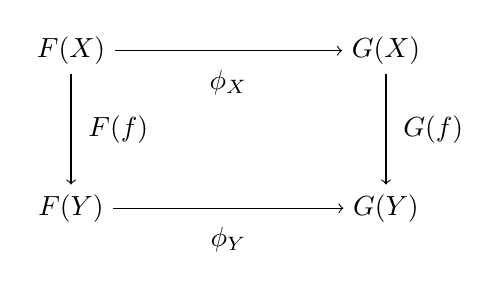
\begin{tikzpicture}
	
	
	
	\node (w) at (0,0) {\(F(X)\)};
	
	\node (x) at (0,-2) {\(F(Y)\)};
	
	\node (y) at (4,-2) {\(G(Y)\)};
	
	\node (z) at (4,0) {\(G(X)\)};
	
	\node (f) at (2,-2.4){\(\phi_Y\)};
	
	\node (g) at (2,-0.4){\(\phi_X\)};
	
	\node (s) at (0.6,-1) {\(F(f)\)};
	
	\node (s2) at (4.6,-1) {\(G(f)\)};	
	
	\draw[->] (z) -- (y);
	\draw[->] (w) -- (x);
	\draw[->] (x) -- (y);
	\draw[->] (w) -- (z);
	
	
	\end{tikzpicture}
	$$
	
	or in other words $\phi_Y \circ F(f) = G(f) \circ \phi_X $ holds.
	
\end{enumerate}
\end{maar}


Next we will define the concepts of limit and colimit for arbitrary categories, which will be later applied to directed and inverse systems.

\begin{maar}
	Let $C$ and $J$ be categories, then we say that the category $C$ is indexed by the category $J$ if there exists a functor $F:J \rightarrow C$.	
\end{maar}	
We call the functor $F$ described above an indexed functor. Because the functor $F$ has the information about the domain $J$ and the range $C$, we can treat functor $F$ as the subcategory $F(J)$ of $C$.
\begin{maar}
Let $C$ be a category indexed by $J$ and let $F:J \rightarrow C$ be the indexing functor. Let $N$ be fixed object of the category $C$. We define the cone from $N$ to $F$ to be an indexed family of morphisms $$\Omega_N = \{\omega_X: N \rightarrow F(X)\}_{X \in J}$$ which satisfies following property: If $f:X \rightarrow Y$ is a morphism in $C$ then the following diagram commutes


$$
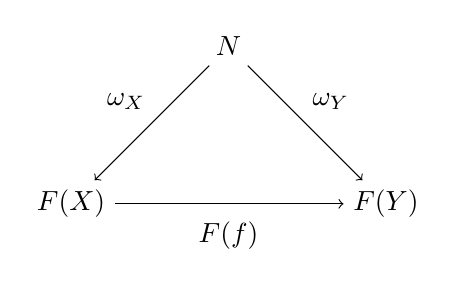
\begin{tikzpicture}

\node (w) at (2,0) {\(N\)};

\node (x2) at (0.7,-0.7) {\(\omega_X\)};

\node (x) at (0,-2) {\(F(X)\)};

\node (y2) at (3.3,-0.7) {\(\omega_Y\)};

\node (y) at (4,-2) {\(F(Y)\)};

\node (f) at (2,-2.4){\(F(f)\)};


\draw[->] (w) -- (y);
\draw[->] (w) -- (x);
\draw[->] (x) -- (y);


\end{tikzpicture}
$$
From now on we will denote the cone structure described above by $\bigtriangleup(F, N, \Omega_N)$. 
\end{maar}

\begin{maar}
Let $C$ be a category which is indexed by a category $J$ and let $F$ be the indexing functor. We say the object $D \in \ob(C)$ is a limit of the functor $F$ if following conditions are satisfied:
\begin{enumerate}[label=(\arabic*),ref=(\arabic*)]
\item There exists family of morphisms $\Omega_D$ which induce cone structure $\bigtriangleup(F, D, \Omega_D)$.
\item If $\bigtriangleup(F, N, \phi)$ is any other cone structure, then there exists unique morphism $u:N \rightarrow D$ which makes the following diagram commute. 
\end{enumerate}
\end{maar}
$$
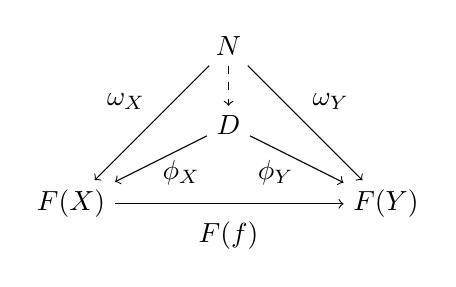
\begin{tikzpicture}

\node (w) at (2,0) {\(N\)};

\node (x2) at (0.7,-0.7) {\(\omega_X\)};

\node (x) at (0,-2) {\(F(X)\)};

\node (y2) at (3.3,-0.7) {\(\omega_Y\)};

\node (y) at (4,-2) {\(F(Y)\)};

\node (f) at (2,-2.4){\(F(f)\)};

\node (d) at (2,-1){\(D\)};

\node (phid) at (1.4,-1.6){\(\phi_X\)};
\node (phid2) at (2.6,-1.6){\(\phi_Y\)};


\draw[->] (w) -- (y);
\draw[->] (w) -- (x);
\draw[->] (x) -- (y);
\draw[dashed][->] (w) -- (d);
\draw[->] (d) -- (x);
\draw[->] (d) -- (y);


\end{tikzpicture}
$$
Next we will prove that if we have two limits $N$ and $D$ of a functor $F$ then there exists an isomorphism between those two objects. In other words $N$ and $D$ can be identified and the limit of functor $F$ can be denoted simply as $\displaystyle {\lim_\rightarrow C}$ .

\begin{lause}
Let $F:J \rightarrow C$ be an indexing functor. Let $N$ and $D$ be limits of a functor $F$. Then there exists an isomorphism between them.
\end{lause}
\begin{proof}
Because $N$ and $D$ are both limits there exists morphisms $u: N \rightarrow D$ and $v: D \rightarrow N $ as above. Because of the symmetry it is enough to show that $u \circ v = id_N$. This follows from the equations $\omega_X \circ u \circ v  = \phi_X \circ u = \omega_X$ and $u \circ v \circ \omega_Y = u \circ \phi_Y = \omega_Y$. Because the diagram commutes for $id_N$ then by the uniqueness condition we see that $u \circ v = id_N$. 
\end{proof}
\subsection{Dual category}
To simplify definitions we will define the concept of dual category. 
\begin{maar}
Let $\omega$ be a statement in this model. We get a dual statement $\omega^{op}$ by following procedure:

\begin{enumerate}[label=(\arabic*),ref=(\arabic*)]
	
	\item Interchange every occurrence of source with target
	\item Reorder every composition. That is replace $a \circ b$ with $b \circ a$.
	
\end{enumerate}
%% Tarkistus suoritettu t�h�n asti
\end{maar}
Next we will give a few important example of a dual statement. 
\begin{maar}
	Let $F:J \rightarrow C$ be the indexing functor. We define cocone to be the dual structure of the cone. 
\end{maar}
We will denote the cocone over object $N$ as $\bigtriangledown(F,N,\Omega_N)$

\begin{maar}
	Let $C$ be a category which is indexed by a category $J$ and let $F$ be the indexing functor. We say the object $D \in \ob(C)$ is a colimit of the functor $F$ if the following conditions are satisfied:
	\begin{enumerate}[label=(\arabic*),ref=(\arabic*)]
		\item There exists family of morphisms $\Omega_D$ which induce cocone structure $\bigtriangledown(F, D, \Omega_D)$.
		\item If $\bigtriangledown(F, N, \phi)$ is any other cone structure, then there exists unique morphism $u:N \rightarrow D$ which makes the following diagram commute. 
	\end{enumerate}
\end{maar}

$$
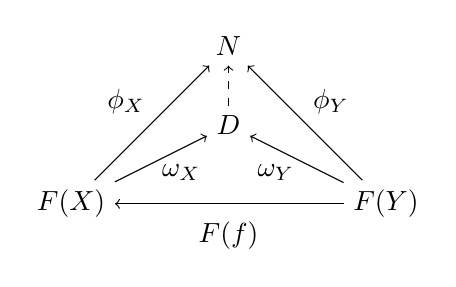
\begin{tikzpicture}

\node (w) at (2,0) {\(N\)};

\node (x2) at (0.7,-0.7) {\(\phi_X\)};

\node (x) at (0,-2) {\(F(X)\)};

\node (y2) at (3.3,-0.7) {\(\phi_Y\)};

\node (y) at (4,-2) {\(F(Y)\)};

\node (f) at (2,-2.4){\(F(f)\)};

\node (d) at (2,-1){\(D\)};

\node (phid) at (1.4,-1.6){\(\omega_X\)};
\node (phid2) at (2.6,-1.6){\(\omega_Y\)};


\draw[->] (y) -- (w);
\draw[->] (x) -- (w);
\draw[->] (y) -- (x);
\draw[dashed][->] (d) -- (w);
\draw[->] (x) -- (d);
\draw[->] (y) -- (d);


\end{tikzpicture}
$$

Like in the case of limits, colimits are unique. 

\begin{lause}
Let $F$ be indexing functor and let $N$ and $D$ be colimits of a functor $F$. Then there exists isomorphism between objects $N$ and $D$.
\end{lause}
\begin{proof}
Because $N$ and $D$ are both colimits there exist morphisms $u: N \rightarrow D$ and $v: D \rightarrow N $ as above. Because of the symmetry it is enough to show that $u \circ v = id_N$ holds. This follows from the equations $u \circ v \circ \omega_X = u \circ \phi_X = \omega_X$ and $u \circ v \circ \omega_Y = u \circ \phi_Y = \omega_Y$. The diagram commutes for $id_N$ and thus by the uniqueness condition we see that $u \circ v = id_N$. 
\end{proof}
\subsection{Direct and inverse systems}
In this section we will give a categorical definition of direct and inverse systems. It appears that those concepts are dual of each other. We will begin by defining quasi-ordering relation:

\begin{maar}
Let $\lambda$ be a category and let $a \leq b$ be a relation in an object class $\ob(\lambda)$. We say that this relation is a quasi-ordering if the following conditions hold:
\begin{enumerate}[label=(\arabic*),ref=(\arabic*)]
	
	
	\item $a \leq a$ for all $a \in \ob(\lambda)$
	\item if $a \leq b$ and $b \leq c$ then $a \leq c$ for all $a,b,c \in \ob(\lambda)$
	
\end{enumerate}

\end{maar}
\begin{maar}
Let $\lambda$ and $C$ be categories and $D:\lambda \rightarrow C$ an indexing functor. We say that functor $D$ is a direct system indexed by $\lambda$ if the following condition hold:
\begin{enumerate}[label=(\arabic*),ref=(\arabic*)]
	
	\item For every pair $a \leq b$ in $\ob(\lambda)$ there exists unique morphism $D^b_a: D(a) \rightarrow D(b)$.
	\item For every triple $a \leq b \leq c$, the morphisms commute in a following way: $D^c_b \circ D^b_a = D^c_a$.
	\item For every $a \in \lambda$: $D^a_a $ is identity morphism $id_a$.
	
\end{enumerate}
\end{maar}

The dual of direct system is inverse system. 

\begin{maar}
Let $\lambda$ and $C$ be categories and $I:\lambda \rightarrow C$ an indexing functor. We say that functor $I$ is an inverse system indexed by $\lambda$ if the following condition hold:
\begin{enumerate}[label=(\arabic*),ref=(\arabic*)]
	
	\item For every pair $a \leq b$ in $\ob(\lambda)$ there exists unique morphism $I^b_a: I(b) \rightarrow I(a)$.
	\item For every triple $a \leq b \leq c$, the morphisms commute in a following way: $I^b_a \circ I^c_b = I^c_a$.
	\item For every $a \in \lambda$: $I^a_a $ is identity morphism $id_a$.
	
\end{enumerate}
\end{maar}

\begin{esim}
Let SET be the category of sets with order relation defined by $U \leq V \Leftrightarrow U \subset V$. Now for every $U,V$ we define $D_U^V: U \rightarrow V $ to be just inclusion from $U$ to $V$. Clearly this forms a direct system. 
\end{esim}

 Earlier we defined the concept of limit for general indexing functors. We can interpret direct and inverse system as indexing functors, taking the $\lambda$ to be indexing set. In general systems the limit may not exist. However, for our purpose it is enough to show that such limit can be found in category of abelian groups.

\begin{lause}
Let $D:\lambda \rightarrow AB$ be a direct system of groups. Let $i_a: D(a) \rightarrow \bigoplus_{a \in \ob(\lambda)} D(a)$  let $G$ be the subgroup of $D = \bigoplus_{a \in \lambda} D(a) $ with is generated by $\{i_ax_{a}-i_bD^b_ax_a\}$. Then the colimit of this system is an object $L = \bigoplus_{a \in \lambda} D(a) / G $.
\end{lause}
\begin{proof}
We denote $p$ to be the projection map: $p: \bigoplus_{a \in \ob(\lambda)} D(a) \rightarrow L$. Let $v$ be the family of morphisms $ \{v_a = p \circ i_a:D(a) \rightarrow L\}_{a \in \ob(\lambda)}$ which induces cocone $\triangledown(I,L,v)$ and let $K$ be any other object with family of morphisms $\phi = \{\phi_a:D(a) \rightarrow K\}_{a \in \ob(\lambda)}$ which induces cocone  $\triangledown(I,K, \phi)$. We have to prove that there exists unique homomorphism $u:L \rightarrow K$ for which condition $u \circ v_a = \phi_a $ holds for all $a \in \ob(\lambda)$. We will first show that such homomorphism exists \newline
Using lemma \ref{Universalpropertysum} we can find unique homomorphism $u':\bigoplus_{a \in \lambda} D(a) \rightarrow K$ for which $u' \circ i_a = \phi_a$ holds. Now we see that for every generator of subgroup G the following equations hold: $$u'(i_ax_{a}-i_bD^b_ax_a) = \phi_a(x_a) - \phi_bD_a^bx_a = \phi_a(x_a)-\phi_a(x_a) = 0.$$ Now we can define $u$ in such way that it maps every element $x + D$ to element $\phi'(x)$. We will denote the projection map from $\bigoplus_{a \in \lambda} D(a)$ to $L$ by $p$. Now we see that $$u \circ v_a = u \circ p \circ i_a = u' \circ i_a = \phi_a.$$
To prove that the homomorphism $u$ we notice that if $x \in L$ , then $x = \sum_{a \in A \subset D} v_a(x_a) + G$. Let $x$ be arbitrary element then, the following equations hold  $$u(x) = u(\sum_{a \in A \subset D}v_a(x_a)) = \sum_{a \in A \subset D} u \circ v_a (x_a) = \sum_{a \in A \subset D} \phi_a(x_a)$$
Thus $u(x)$ is determined by the sum of homomorphisms $\phi_a$. It follows that the map $u$ is unique.
\end{proof}
\begin{lause}
Let $I: \lambda \rightarrow AB$ be a inverse system of groups. Then the limit of this functor is group $L = \{x \in \prod_{i \in J} I_i \mid x_a = I^b_ax_b $ for all $a \leq b\}$
\end{lause}
\begin{proof}
Let  $v$ be a family of homomorphisms $\{v_a = pr_a: L \rightarrow I(a)\}_{a \in \lambda}$ which together with group $L$ induce cone $\bigtriangleup(I,L,v)$. Let $K$ be any other group and let be family of homomorphisms $\phi = \{\phi_a: K \rightarrow I(a)\}_{a \in \lambda}$ which induces cone $\bigtriangleup(I,K,\phi)$ . \newline 
We construct function $u: K \rightarrow L$ for which $v_a \circ u = \phi_a$ holds. Using lemma \ref{Universalpropertyproduct} we find unique homomorphism $u':K \rightarrow \prod_{i \in J}I_i$ for which $pr_a \circ u' = \phi_a$ is satisfied. Let $u''$ be the homomorphism, where the image is restricted to subgroup $L$. We will show that the homomorphism is well-defined, specifically $u'$ maps every element inside the subgroup $L$. Assume that $b$ and $a$ are elements which satisfy $a \leq b$ condition. Then the following equation hold $$I^{b}_a \circ pr_b \circ u'= I^{b}_a \circ \phi_b = \phi_a = pr_a \circ u'.$$ We can define $u$ to be $u''$. The uniqueness property of the homomorphism follows directly from the fact that $u'$ is unique. 
\end{proof}

\subsection{Morphisms between systems}\label{limitmorphism}
\subsubsection{Morphisms between inverse systems}

To be able to define morphisms between Cech homology groups we need the concept of a limit homomorphism. In this section we will define limit morphism between systems and investigate properties of it. Concepts used in this chapter can be presented in a more general way. However, for our use case its enough to restrict ourselves to the direct and inverse system.

\begin{maar}
Functor $\phi:X \rightarrow Y$ is order preserving if for every elements $a$ and $b$ in set $X$ for which $a \leq b$, the condition $\phi(a) \leq \phi(b)$ is satisfied.
\end{maar}
 Let $I$ be inverse system and $\phi: \lambda' \rightarrow \lambda$ order preserving functor. Then inverse system $(I \phi, \lambda' )$ consist of objects $\{I'(\phi(a)) \mid a \in \ob(\lambda')\}$ and morphisms $\{I^{\phi(b)}_{\phi(a)}\mid a \leq b \}$.


\begin{maar}
Let $(I,\lambda)$ and $(I',\lambda')$ be inverse systems and $\phi:\lambda' \rightarrow \lambda$ an order and limit preserving functor. Let $ \{f_a:I(\phi(a)) \rightarrow I'(a) \mid a \in \lambda\}$ be natural transformation between $I\phi$ and $I'$. Then we say that $\{f_a\}_{a \in \lambda}$ is an inverse system of morphisms corresponding to functor $\phi$ of the system $I$ into system $I'$.
\end{maar}

In next theorem we prove that it is possible to define limit of the morphism between systems in an unique way. We recall that exists of limit implies that for every objects of category $I$ there exists unique functor $u_{I,a}:\lim I \rightarrow I(a)$.

\begin{lem}
Let  $(I,\lambda)$ and $(I',\lambda')$ be inverse systems for which limit exists. Let $\{f_a\}$ be inverse system of morphisms corresponding to that pair. Then there exists unique morphism $\lim f:\lim I \rightarrow \lim I'$ for which and for every $a \in \lambda'$ condition $\lim f \circ u_{I, \phi(a)} = u_{I',a} \circ f_a$ holds.
\end{lem}
\begin{proof}
Consider following diagram
\begin{diagram}\label{morphismbetweenlimits}
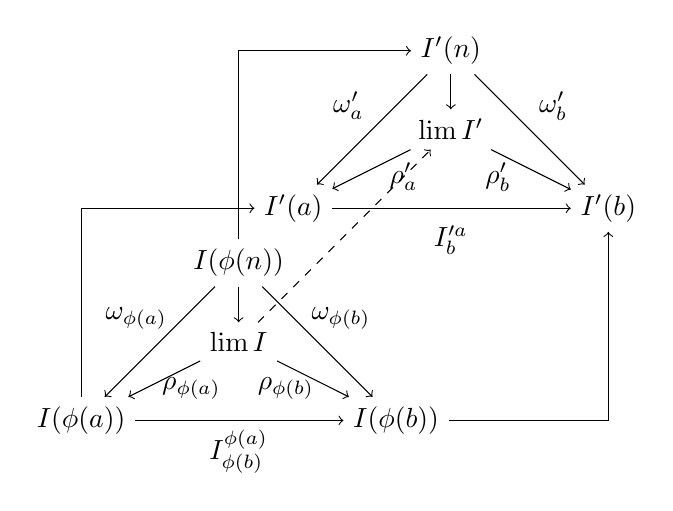
\begin{tikzpicture}

\node (w) at (2,0,0) {\(I(\phi(n))\)};

\node (x2) at (0.7,-0.7,0) {\(\omega_{\phi(a)}\)};

\node (x) at (0,-2,0) {\(I(\phi(a))\)};

\node (y2) at (3.3,-0.7,0) {\(\omega_{\phi(b)}\)};

\node (y) at (4,-2,0) {\(I(\phi(b))\)};

\node (f) at (2,-2.4,0){\(I^{\phi(a)}_{\phi(b)}\)};

\node (d) at (2,-1,0){\(\lim I\)};

\node (phid) at (1.4,-1.6,0){\(\rho_{\phi(a)}\)};
\node (phid2) at (2.6,-1.6,0){\(\rho_{\phi(b)}\)};

\node (w2) at (2,0,-7) {\(I'(n)\)};

\node (x22) at (0.7,-0.7,-7) {\(\omega'_a\)};

\node (x2) at (0,-2,-7) {\(I'(a)\)};

\node (y22) at (3.3,-0.7,-7) {\(\omega'_b\)};

\node (y2) at (4,-2,-7) {\(I'(b)\)};

\node (f2) at (2,-2.4,-7){\(I'^{a}_{b}\)};

\node (d2) at (2,-1,-7){\(\lim I'\)};

\node (phid2) at (1.4,-1.6,-7){\(\rho'_a\)};
\node (phid22) at (2.6,-1.6,-7){\(\rho'_b\)};

\draw[->] (w) -- (y);
\draw[->] (w) -- (x);
\draw[->] (x) -- (y);
\draw[->] (w) -- (d);
\draw[->] (d) -- (x);
\draw[->] (d) -- (y);

\draw[->] (w2) -- (y2);
\draw[->] (w2) -- (x2);
\draw[->] (x2) -- (y2);
\draw[->] (w2) -- (d2);
\draw[->] (d2) -- (x2);
\draw[->] (d2) -- (y2);

\draw[->] (w) |- (w2);
\draw[->] (x) |- (x2);
\draw[->] (y) -| (y2);


\draw[dashed][->](d) -- (d2);


\end{tikzpicture}
\end{diagram}

To prove that the limit morphism exists we form following triangle out of the diagram described above:

$$
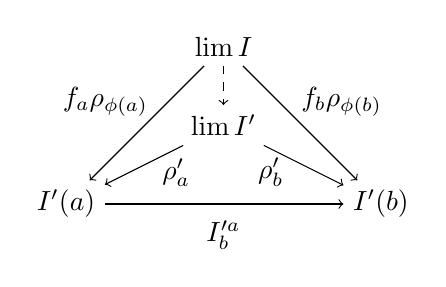
\begin{tikzpicture}

\node (w) at (2,0) {\(\lim I\)};

\node (x2) at (0.5,-0.7) {\(f_a \rho_{\phi(a)}\)};

\node (x) at (0,-2) {\(I'(a)\)};

\node (y2) at (3.5,-0.7) {\(f_b \rho_{\phi(b)}\)};

\node (y) at (4,-2) {\(I'(b)\)};

\node (f) at (2,-2.4){\(I'^{a}_{b}\)};

\node (d) at (2,-1){\(\lim I'\)};

\node (phid) at (1.4,-1.6){\(\rho'_a\)};
\node (phid2) at (2.6,-1.6){\(\rho'_b\)};


\draw[->] (w) -- (y);
\draw[->] (w) -- (x);
\draw[->] (x) -- (y);
\draw[dashed][->] (w) -- (d);
\draw[->] (d) -- (x);
\draw[->] (d) -- (y);


\end{tikzpicture}
$$
Then by definition of limit there exists unique morphism $\lim f:\lim I \rightarrow \lim I'$ for which the diagram commutes. We will prove now that the universal property $\lim f \circ u_{I, \phi(a)} = u_{I',a} \circ f_a$ holds for limit morphism. By diagram \ref{morphismbetweenlimits} and fact that the family of function $\{f_a\}$ is natural transformation or in other words condition $\omega'_a \circ f_n = f_a \circ \omega_{\phi(a)}$ holds following diagram commutes:
$$
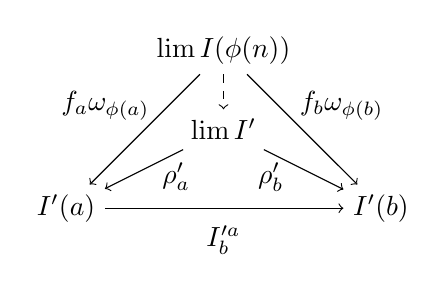
\begin{tikzpicture}

\node (w) at (2,0) {\(\lim I(\phi(n))\)};

\node (x2) at (0.5,-0.7) {\(f_a \omega_{\phi(a)}\)};

\node (x) at (0,-2) {\(I'(a)\)};

\node (y2) at (3.5,-0.7) {\(f_b \omega_{\phi(b)}\)};

\node (y) at (4,-2) {\(I'(b)\)};

\node (f) at (2,-2.4){\(I'^{a}_{b}\)};

\node (d) at (2,-1){\(\lim I'\)};

\node (phid) at (1.4,-1.6){\(\rho'_a\)};
\node (phid2) at (2.6,-1.6){\(\rho'_b\)};


\draw[->] (w) -- (y);
\draw[->] (w) -- (x);
\draw[->] (x) -- (y);
\draw[dashed][->] (w) -- (d);
\draw[->] (d) -- (x);
\draw[->] (d) -- (y);


\end{tikzpicture}
$$
Both maps $\lim f \circ u_{I, \phi(a)}$ and $u_{I',a} \circ f_a$ complete the diagram. Thus by uniqueness of the map corresponding to limit, we can conclude that the functions are same.

\end{proof}
For composition of two limits we have following result:

\begin{lem}\label{compositionlimitmorphism}
Let $(I, \lambda)$, $(I',\lambda')$ and $(I'',\lambda'')$ be inverse systems with limits and let $\phi:\lambda' \rightarrow \lambda$ and $\phi':\lambda'' \rightarrow \lambda'$ functors between systems. Let $ \{f_a:I(\phi(a)) \rightarrow I'(a) \mid a \in \phi'(\lambda'')\}$ and $ \{g_a:I'(\phi(a)) \rightarrow I''(a) \mid a \in \lambda''\}$ be family of morphisms corresponding to $\phi$ and $\phi'$. Let $\lim(f \circ g):I \rightarrow I''$ be limit of the family $\{g_af_{\phi(a)}:I(\phi \phi'(a)) \rightarrow I''(a) \mid a \in \lambda''\}$.  Then $\lim(f \circ g) = \lim f \circ \lim g $ holds.
\end{lem}
\begin{proof}
To prove this we will use previous lemma and following commutable diagram:
	$$
	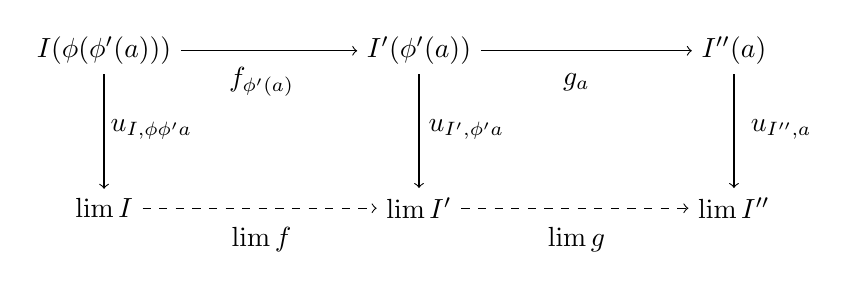
\begin{tikzpicture}
	
	
	
	\node (w) at (0,0) {\(I(\phi(\phi'(a)))\)};
	
	\node (x) at (0,-2) {\(\lim I\)};
	
	\node (y) at (4,-2) {\(\lim I'\)};
	
	\node (z) at (4,0) {\(I'(\phi'(a))\)};
	
	\node (p) at (8,0) {\(I''(a)\)};
	
	\node (p2) at (8,-2) {\(\lim I''\)};
	
	\node (f) at (2,-2.4){\(\lim f\)};\
	
	\node (f2) at (6,-2.4){\(\lim g\)};
	
	\node (g) at (2,-0.4){\(f_{\phi'(a)}\)};
	
	\node (g2) at (6,-0.4){\(g_{a}\)};
	
	\node (s) at (0.6,-1) {\(u_{I,\phi \phi'a}\)};
	
	\node (s2) at (4.6,-1) {\(u_{I', \phi'a}\)};	
	
	\node (s3) at (8.6,-1) {\(u_{I'', a}\)};	
	
	\draw[->] (z) -- (y);
	\draw[->] (w) -- (x);
	\draw[dashed][->] (x) -- (y);
	\draw[->] (w) -- (z);
	\draw[dashed][->] (y) -- (p2);
	\draw[->] (p) -- (p2);
	\draw[->] (z) -- (p);
	
	
	\end{tikzpicture}
	$$
	By definition of limit morphism condition $\lim (f \circ g) \circ u_{I, \phi(\phi'(a))} = u_{I'',a} \circ (g_a \circ f_{\phi(a)})$ holds for limit of the composition. By uniqueness of limit homomorphism it is enough to show that the composition of two limit functors satisfies the condition. This follows from following equations:
	$$\lim g \circ \lim f \circ u_{I, \phi(\phi'(a))} = \lim g  \circ u_{I, \phi'(a)} \circ f_{\phi'(a)} = u_{I'',a} \circ g_a \circ f_{\phi(a)} $$
	

\end{proof}

Now we would like to define limit for the system of homomorphisms between inverse systems of groups.

\begin{lem}\label{limitmorphismgroup}
Let $(I, \lambda)$ and $(I',\lambda')$ be inverse systems of groups. Then $$f:\lim_{\rightarrow} I \rightarrow \lim_{\rightarrow}I' : f(x) = \prod_{a \in \lambda}f_a(proj_{\phi(a)}(x))$$
is well defined function between limit groups.
\end{lem}
\begin{proof}
We have to show that the image is in the subgroup $$L = \{x \in \prod_{i \in \lambda'} I'(i) \mid x_a = I^b_ax_b \text{ for all } a \leq b \}.$$ Let $b$ be some index, then: $I'^{b}_{a}x'_b = I'^{b}_{a}f_b(x_{\phi(b)}) = f_bI'^{\phi(b)}_{\phi(a)}(x_{\phi(b)}) = f_ax_{\phi(a)} = x'_a$ . In this equation we used property which says that the morphisms define natural transformation.
\end{proof}

\subsection{Finality properties of subsystems}
Final and cofinal functors can be defined in a more general way [\ref{categorytheory}]. However, because we are mainly interested in properties of systems, in this section we will investigate the properties of those specific functors only in that special case. In the case of general categories, cofinality included a concept of connectedness defined in [\ref{categorytheory}] page 217. In our definition we will use a stronger version of that concept.

%% continue here:
\begin{maar}
Let $\lambda$ be a category with quasi-order relation on its objects and let $\lambda'$ be its subcategory. Then we say that $\omega$ is cofinal subcategory of $\lambda$, if for every two objects $a,b \in \ob(\lambda)$ there exist element in $t \in \ob(\lambda')$ in such a way that conditions $a \leq t$ and $b \leq t$ hold.
\end{maar}

Now for the inverse system we have following theorem:

\begin{lause}
Let $(I,\lambda)$ be inverse system and let $(I',\lambda')$ be its subsystem generated by connected cofinal subcategory $\lambda$. Assume that there exists limit object for $I'$. Then the limit of the system $(I,\lambda)$ is $\lim I'$.

\end{lause}
\begin{proof}
Let $\lim I'$ be limit of inverse system $I'$. It is enough to show that $\lim I'$ is also the limit of $I$. We will first show that $\lim I'$ forms a cone in $I$ and then prove that for any other cone induced by object $N$ in $I$ there exists unique morphism $u:N \rightarrow \lim I'$ \newline
 Let $I(b$ be arbitrary object of inverse system $I$. Then by definition of cofinal subcategory there exists element $a' \in I'$ for which $a \leq a'$ holds. Thus there exists a morphisms $I^{a'}_a$. Because $\lim I'$ is limit of inverse system $I'$ it forms cone $\bigtriangleup(I',\lim I',\rho)$, where $\rho$ is some collection of morphisms $\{\rho_{a}: \lim I' \rightarrow I'(a)\}_{a \in \ob(\lambda')}$. Using $\rho$ we form a new collection of morphisms $\rho'$ defined by $\{I^{a'}_a \circ \rho_{a'}:\}_{a \in \ob(\lambda)} $. Because $I^{a'}_a \circ \rho_{a'}$ can vary on the choice of $a$, the composition may be not uniquely determined. However, if $a''$ is another element for which relation $a \leq a''$ holds, then there exists element $t$ for which conditions $a \leq t$ and $a'' \leq t$ are satisfied. Because the following equations hold $$I^{a'}_a \circ \rho_{a'} = I^{a'}_a \circ I^{t}_{a'} \circ \rho_t = I^t_a \circ \rho_t = I_a^{a''} \circ I^{t}_{a''} \circ \rho_{t} = I^{a''}_a \circ p_{a''}$$ 
 we can conclude that $I^{a'}_a \circ \rho_{a'} = I^{a''}_a \circ p_{a''}$ and thus the family of the homomorphisms is well-defined and $\lim(I')$ forms a cone $\bigtriangleup(I,\lim I', \rho' )$\newline
 Now if there exists another cone $\bigtriangleup(I,N,\omega)$ , we have construct map $u:N \rightarrow \lim I'$ and prove that it is unique. Let $a$ and $b$ be objects of $\lambda$, then there exists objects $a'$ and $b'$ for which relations $a \leq a'$ and $b \leq b'$ hold. Restricting collection $\omega$ to the morphisms indexed by $\lambda'$ we get cone $\bigtriangleup(I',N,\omega')$ of $I'$. Because $\lim I'$ is the limit of the functor $I'$, there exists a unique homomorphism $u:N \rightarrow \lim I'$. It is left to prove that following diagram commutes:
  $$
 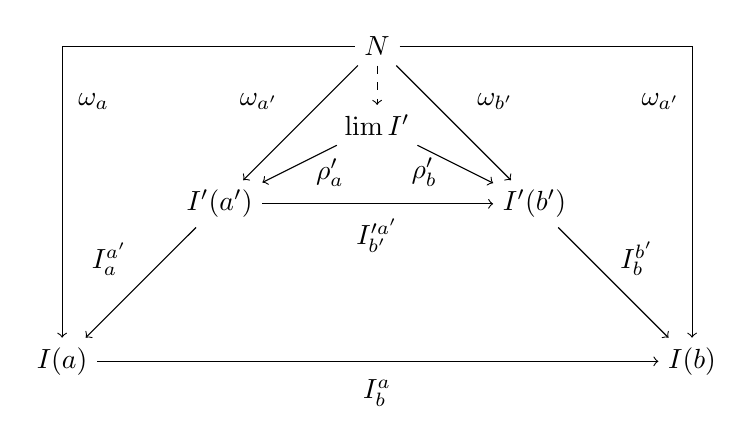
\begin{tikzpicture}
 
 \node (w) at (2,0) {\(N\)};
 
 \node (x2) at (0.5,-0.7) {\(\omega_{a'}\)};
 
  \node (x3) at (-1.6,-0.7) {\(\omega_{a}\)};
 
 \node (a2) at (-1.4,-2.7) {\(I^{a'}_{a} \)};
 
 \node (x) at (0,-2) {\(I'(a')\)};
 
 \node (y2) at (3.5,-0.7) {\(\omega_{b'}\)};
 
   \node (y3) at (5.6,-0.7) {\(\omega_{a'}\)};
 
  \node (b2) at (5.3,-2.7) {\(I^{b'}_{b} \)};
 
 \node (y) at (4,-2) {\(I'(b')\)};
 
 \node (f) at (2,-2.4){\(I'^{a'}_{b'}\)};
 
  \node (f2) at (2,-4.4){\(I^{a}_{b}\)};
 
 \node (d) at (2,-1){\(\lim I'\)};
 
 \node (phid) at (1.4,-1.6){\(\rho'_a\)};
 \node (phid2) at (2.6,-1.6){\(\rho'_b\)};
 
 \node(a) at (-2,-4) {\(I(a)\)};
  \node(b) at (6,-4) {\(I(b)\)};
 
 \draw[->] (w) -- (y);
 \draw[->] (w) -- (x);
 \draw[->] (x) -- (y);
 \draw[dashed][->] (w) -- (d);
 \draw[->] (d) -- (x);
 \draw[->] (d) -- (y);
 \draw[->] (x) -- (a);
 \draw[->] (y) -- (b);
 \draw[->] (a) -- (b);
 \draw[->] (w) -| (a);
 \draw[->] (w) -| (b);
 
 
 
 \end{tikzpicture}
 $$
 Especially we have to prove that $I^{a'}_{a} \circ w_{a'} = w_a $ . This claim follows directly from the fact that $\bigtriangleup(I,N,\omega) $ is a cone. Thus the $u$ defined above is the map we were searching for.

\end{proof}


\section{Nerve of covering}
In this chapter we will give abstract definition of simplicial complex. 


\subsection{Abstract simplicial complex}
We assume that reader knows already basic facts about simplicial complexes if not we suggest to take a look at [\ref{rotman}]. We start by defining infinite dimensional simplicial complex.

\begin{maar}
Let $X$ be a set and $S = \{S_i\}_{i \in J}$ be some finite collection of subsets of the set $X$. We say that $S$ forms abstract simplicial complex over $X$, if subset of any set $S_i$ in the collection $S$ is in the collection.
\end{maar}
For abstract simplicial complex we define following geometric structure which will give us the interface of original simplicial complex.
\begin{maar}
The geometric $\mathcal{S}(X)_S$ realization of the abstract simplicial complex is a subset of the set $[0,1]^X$ for which the following conditions are satisfied: Let $x \in \mathcal{S}(X)$ then
\begin{enumerate}[label=(\arabic*),ref=(\arabic*)]
	\item Relation $pr_i(x) > 0$ holds only for finitely many indexes $i \in J$.
	\item $\sum_{i \in J}pr_i(x) = 1$.
	\item Set $\{i \in J \mid pr_i(x) > 0\}$ belongs to collection $S$.
\end{enumerate}

\end{maar}
\begin{lem}
Let $X$ be a set and $S = \{S_i\}_{i \in J}$ be some collection of subsets of the set $X$. Let $\mathcal{S}(X)_S$ be its geometric realization. Then $\mathcal{S}(X)_S$ is simplicial complex.
\end{lem}
\begin{proof}
We define collection simplexes of the simplicial complex to be the geometric realizations of sets $S_i$ in the collection. Any face is in the collection by definition of abstract simplicial complex. Also any intersection of two simpleces is in the collection. Thus $\mathcal{S}(X)_S$ is simplicial complex.
\end{proof}
\begin{maar}
Let set $X$ together with collection $S = \{S_i\}_{i \in I}$ be abstract simplicial. Let $A$ be some subset of $X$ and $S' = \{S'_i\}_{i \in I}$ some collection of its subsets. Then we say that $\mathcal{S}(A)_{S'}$ is subsimplex of $\mathcal{S}(X)_S$.
\end{maar}
If $\mathcal{S}(X)$ is simplicial complex and $\mathcal{S}(A)$ its subcomplex they form topological pair which we will denote by $(\mathcal{S}(X)_S, \mathcal{S}(A)_{S'})$  Next we will recall the definition of simplicial map.
\begin{maar}
Let $(X,A)$ and $(Y,B)$ be simplicial complexes and $f$ map between pairs. Then we say that map $f$ is simplicial if for any simplex in $X$ the images of vertexes of the simplex span some simplex in $Y$ and images of vertexes of simplex in $A$ span some simplex in $B$.
\end{maar}
\begin{maar}
Let $f:(X,A) \rightarrow Y$ and $g:(X,A) \rightarrow (Y,B)$ be simplicial maps then we say that maps are contiguous if for every simplex $s = \{a_1, ..., a_n\}$ in $X (A)$ there exists simplex $k$ in $Y (B)$ for which span$(f(a_1), ..., f(a_n)) \subset k$ and span$(g(a_1), ..., g(a_n)) \subset k $ 
\end{maar}
\begin{lem}
If $f:(X,A) \rightarrow (Y,B)$ and $g:(X,A) \rightarrow (Y,B)$ are contiguous maps then they are homotopic.
\end{lem}
\begin{proof}
We define $H:X \times [0,1] \rightarrow Y$ in a following way:  $$H(x,t) = tf(x)+(1-t)g(x)$$
It is easy to see that $H(x,0) = f(x)$ and $H(x,1) = g(x)$, also because $f(x)$ and $g(x)$ both belong to same simplex $H(x,t)$ is well defined at every point. 
\end{proof}
\subsection{Coverings}
We begin by recalling definition of covering
\begin{maar}
Let $X$ be a topological space and $\{A_i\}_{i \in J}$ collection of its open subsets. Then we say that  $\{A_i\}_{i \in J}$ is covering of $X$ if $\bigcup_{i \in J}A_i = X$.
\end{maar}
We will denote set of all open coverings of space $X$ by COV$(X)$. Because in homology we are interested in pair of spaces we give definition of covering for the pair. 
\begin{maar}
Let $(X,A)$ be topological pair. Then we say that $\{(U_i, V_i )\}_{i \in J}$ is covering of $(X,A)$ if $V_i \subset U_i$ , $\{U_i\}_{i \in J}$ covers $X$ and $\{V_i\}_{i \in J}$ covers $A$. 
\end{maar}
Respectively we will define set of all coverings of pair $(X,A)$ to be  COV$(X,A)$. Now we are ready to define nerve of the covering. 
\begin{maar}
Let $(U_i,V_i)_{i \in J}$ be covering of some topological pair $(X,A)$. Then nerve of this covering is following abstract simplicial complex $\mathcal{S}(X,A)$:  
\begin{enumerate}[label=(\arabic*),ref=(\arabic*)]
\item We define vertex set of the complex $\mathcal{S}(X)$ to be $\{U_i\}_{i \in J}$ and vertex set of subcomplex $\mathcal{S}(A)$ to be $\{V_i\}_{i \in J}$. 
\item Let $I \subset J$, then for every such $I$ for which $\bigcap_{i \in I}U_i \neq \emptyset$ define simplex in simplicial complex $\mathcal{S}(X)$. In other words $\mathcal{S}(X)$ consist of simplexes defined by all non-empty intersection of spanning sets. In subcomplex $\mathcal{A}$ we define simplex for every non-empty intersection $\bigcap_{i \in I}V_i \cap A$ where $I$ is some subspace of $J$.
\end{enumerate}
\end{maar}
It is easy to see that the simplicial complex is well defined. We can interpret simplicial complex $\mathcal{S}(X)$ as collection of faces of one big complex, then it is enough to show that every face of any simplexes in the collection belongs to the collection. We see that if  $\bigcap_{i \in N}U_i \neq \emptyset$, then for every $M \subset N$ intersection of $\bigcap_{i \in M}U_i $ is non empty. In coverings of topological pair $(X,A)$ we can define quasi order in a natural way. First we will recall definition of refinement.
\begin{maar}
Let $\alpha = \{(U_i,V_i)\}_{i \in I}$ and $\beta = \{(U'_i,V'_i)\}_{i \in J}$ be coverings of some pair $(X,A)$. Then covering $\beta$ is called refinement of $\alpha$ if for every $(U'_i,V'_i) \in \beta$ there exists some $(U_i,V_i) \in \alpha$ for which $U'_i \subset U_i$   and $V'_i \subset V_i$.
\end{maar}
Now we are ready to define the quasi order in the collection of coverings of an arbitary topological space.
\begin{lem}
Let $\text{COV}(X,A)$ be collection of all coverings of the pair $(X,A)$, then order defined by $\alpha \leq \beta$ if and only if $\beta$ is refinement of $\alpha$ is quasi-order.
\end{lem}
\begin{proof}
	Any covering is refinement of itself and if we $a \leq b$ and $b \leq c$ then for every set $U_c$ we can find $U_b$ for which $U_c \subset U_b$ and $U_b \subset U_a$ for some $U_a$. Then we see that $U_c \subset U_a$  so actually $c$ is refinement of $a$. 
\end{proof}
 
\begin{maar}
Let $\beta$ and $\alpha$ be coverings for which $\alpha \leq \beta$. Then we define $\mathcal{P}(\alpha, \beta)$ to be collection of the following projection maps $p^\beta_\alpha:\beta \rightarrow \alpha$: Every $U_i \in \beta$ is mapped to some set $U'_i \in \alpha$ for which $U_i \subset U_i'$ holds.
\end{maar}
We will now show that the family of projection maps is closed under composition.
\begin{lem}\label{compofprojmaps}
	Let $p^\beta_\alpha$ and $p^\gamma_\beta$ be some projection maps . Then $p^\beta_\alpha \circ p^\gamma_\beta$ is also projection map.
\end{lem}
\begin{proof}
	Let $U \in \gamma$, then there exists $U' \in \beta$ and $U'' \in \alpha $ for which condition $U \subset U' \subset U''$ is satisfied. By properties of inclusion $U \subset U''$ and thus $p^\beta_\alpha \circ p^\gamma_\beta$ is a projection map.
\end{proof}
\begin{lem}
The collection of coverings $\text{COV}(X,A)$ is a category defined in the following way:
\begin{enumerate}[label=(\arabic*),ref=(\arabic*)]
	\item The objects of $\text{COV}(X,A)$ are all open coverings of the pair $(X,A)$.
	\item We define $\text{Hom}(\beta,\alpha)$ to be $\mathcal{P}(\alpha, \beta)$, if $\alpha \leq \beta$. Else we define $\text{Hom}(\beta,\alpha)$ to be empty set.  
	\item The composition of maps is defined to be the usual composition of functions.

\end{enumerate}
\end{lem}
\begin{proof}
By lemma \ref{compofprojmaps} the composition of two projection maps is projection map and thus is well-defined. For every $\alpha$ there exists well-defiend projection map $p^{\alpha}_{\alpha}$ which acts like identity map on the $\text{COV}(X,A)$. The associativity condition holds, because every morphism is a function.
\end{proof}
\begin{maar}
Let $F:(X,A) \rightarrow (Y,B)$ and let $\beta$ be covering of $(Y,A)$, then define $f^{-1}\beta$ to be covering of $(X,A)$ which is induced by elements $(f^{-1}U_i, f^{-1}V_i)_{i \in J_{\beta}}$.
\end{maar}
\begin{lem}
Let $F:(X,A) \rightarrow (Y,B)$ be function between pairs and let $\alpha$ and $\beta$ be covers for $(X,A)$ and $(Y,B)$ for which $\alpha = f^{-1}\beta$ holds. Then a map $p: \mathcal{S}(X,A)_{\alpha} \rightarrow \mathcal{S}(Y,B)_{\beta}$ defined by $(f^{-1}U_i, f^{-1}V_i) \rightarrow (U_i, V_i)$ is well defined.
\end{lem}
\begin{proof}
Let $\bigcap_{i \in I}f^{-1}U_i \neq \emptyset$ for some index set $I \subset J$ . We see that $\bigcap_{i \in I}U_i \neq \emptyset$, so the lemma holds.
\end{proof}
\begin{lem}
Let $\beta$ and $\alpha$ be coverings of $(X,A)$ in such way that $\alpha \leq \beta$ and $p$ be a projection map belonging to $\mathcal{P}(\alpha,\beta)$. Let map $p'^\beta_\alpha:\mathcal{S}(X,A)_\beta \rightarrow \mathcal{S}(X,A)_\alpha$ be a map between simplices defined by edges $U \in \mathcal{S}(X,A)_\beta$ with requirment of being piecewise linear on the other elements. Then the map $p'$ is well-defined.
\end{lem}
\begin{proof}
Let $x$ be arbitary element of $\mathcal{S}(X,A)_\beta$, then it belongs to some simplex. Let $S$ be simplex which is intersection of all simplices in $\mathcal{S}(X,A)_\beta$ which have property that intersection with $\{x\}$ is non-empty. In simplex $S$ point $x$ has unique representation $x = \sum_{i \in J}r_ia_i$ where elements $a_i$ are edges and $r_i$ such non-negative real numbers for which $\sum_{i \in J}r_i = 1$. By definition of map $p'$ this point is mapped to $p'(x) = \sum_{i \in J}r_ip^\beta_\alpha(a_i) $ which is uniquely determined so map $p'$ is well-defined.
\end{proof}

We denote map $p'^\beta_\alpha$ described above just as $p^\beta_\alpha$. It is clear from context which of the maps is being used. We will prove now that the map $p$ is simplicial 

\begin{lem}
Projection maps $p^\beta_\alpha$ are simplicial.
\end{lem}
\begin{proof}
Let $s$ be simplex in $\mathcal{S}(X,A)_\alpha$ spanned by some sets $\{U_i\}_{i \in J}$ for which $\bigcap_{i \in J}U_i \neq \emptyset $. Every $U_i$ is mapped to some vertex $U_i'$ in $\mathcal{S}(X,A)_\beta$ for which $U_i \subset U_i'$. Intersection $\bigcap_{i \in J}U'_i$ is clearly non empty, so every simplex is mapped inside some simplex. \newline	
\end{proof}
Projection maps are not uniquely determined by coverings $\alpha$ and $\beta$, but any of those maps are contiguous thus they define same homology groups.
\begin{lem}
Let $\alpha$ and $\beta$ be any coverings of $(X,A)$ for which condition  $\alpha \leq \beta$ is satisfied. Then projection maps $p^\beta_\alpha$ and $p'^\beta_\alpha$ are contiguous.
\end{lem}
\begin{proof}

To prove that the maps are contiguous we form simplex in $\mathcal{S}(Y,B) $ and prove that images of both maps belong to it. Every vertex $U_i$ in $\mathcal{S}(X,A)$ is mapped to $U'_i$ and $U''_i$ by $p^\beta_\alpha$ and $p'^\beta_\alpha$ respectively. Now if $\bigcap_{i \in J}U_i \neq \emptyset$ then also $\bigcap_{i \in J}U'_i \cap \bigcap_{i \in J}U''_i \neq \emptyset$. In case if the vertexes belong to $\mathcal{S}(A)$ it is easy to see that projection map maps them to some simplex in $\mathcal{S}(B)$.  
\end{proof}
By using this lemma and the fact that contiguous simplicial maps induce same homology groups we can define unique homomorphisms $I^{\beta}_{\alpha}:H_q(\mathcal{S}(X,A)_{\beta}) \rightarrow H_q(\mathcal{S}(X,A)_{\alpha})$ for every $q \in \N$.

For projection maps and induced homomorphisms we have following useful lemma.

\begin{lem}\label{preimageorder}
Let $\alpha$ be covering of pair $(X,A)$ and $\beta$ covering of pair $(Y,B)$ for which $\alpha \leq \beta$ holds and $f:(X,A) \rightarrow (Y,B)$ a function between pairs. Then pre-image $f^{-1}\beta$ of covering $\beta$ is refinement of $f^{-1}\alpha$.
\end{lem}
\begin{proof}
This follows directly from the fact that if $U \subset V$, then also $f^{-1}U \subset F^{-1}V$.

\end{proof}

\begin{lem}\label{squarelemmaforcoverings}
	Let $f:(X,A) \rightarrow (Y,B) $ and $\alpha$ and $\beta$ coverings of $(Y,B)$ for which $\alpha \leq \beta$ holds. Let $p^\beta_\alpha$ be projection map for the coverings, then there exists projection map $p^{\beta'}_{\alpha'} $ for which the the diagram commutes.
		$$
	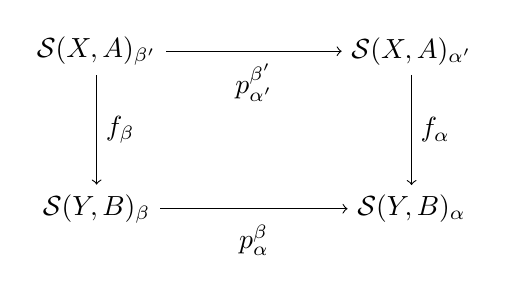
\begin{tikzpicture}
	
	
	
	\node (w) at (0,0) {\(\mathcal{S}(X,A)_{\beta'}\)};
	
	\node (x) at (0,-2) {\(\mathcal{S}(Y,B)_{\beta}\)};
	
	\node (y) at (4,-2) {\(\mathcal{S}(Y,B)_{\alpha}\)};
	
	\node (z) at (4,0) {\(\mathcal{S}(X,A)_{\alpha'}\)};
	
	\node (f) at (2,-2.4){\(p^\beta_\alpha\)};
	
	\node (g) at (2,-0.4){\(p^{\beta'}_{\alpha'}\)};
	
	\node (s) at (0.3,-1) {\(f_{\beta}\)};
	
	\node (s2) at (4.3,-1) {\(f_{\alpha}\)};	
	
	\draw[->] (z) -- (y);
	\draw[->] (w) -- (x);
	\draw[->] (x) -- (y);
	\draw[->] (w) -- (z);
	
	
	\end{tikzpicture}
	$$

\end{lem}

\begin{proof}
Let $\{U_i\}_{i \in J}$ be some simplex in $\mathcal{S}(X,A)_{\beta'}$. For every edge $U$ the set $f^{-1} \circ p \circ f(U) $ is non-empty because $p$ maps $f(U)$ to larger set. Thus for every edge $U_i$ there is corresponding edge in $\mathcal{S}(X,A)_{\alpha'}$. We can now define map $p^{\beta'}_{\alpha'}: \mathcal{S}(X,A)_{\beta'} \rightarrow \mathcal{S}(X,A)_{\alpha}$ in such way that edge $U$ is mapped to the edge $f^{-1}pfU $ and we extend this map by linearity. Now by defining map $p^{\beta'}_{\alpha'}$ in such way for every simplex we get well-defined map for which the diagram commutes.
\end{proof}

\chapter{Cech homology}

In this chapter we will construct Cech homology and prove main results related to it.  We will first define inverse system of homology groups of the nerves.

\begin{maar}
Let $\alpha$ be element of COV$(X,A)$ and $G$ abelian group. Then we can define group $H_{q,a}(X,A;G)$ using the singular homology groups in a following way: $$H_{q,a}(X,A;G) = H_q(\mathcal{S}(X,A)_{\alpha};G)$$. 
For every coverings of $\alpha, \beta$ in $(X,A)$ for which $\alpha \leq \beta$ we define the maps to be
$$I^{\beta}_{\alpha}: H_{q,\beta} \rightarrow  H_{q,\alpha}$$ 
maps $I_{\beta}^{\alpha}$ are induced by some maps $p^\beta_\alpha$ which are unique up to homotopy.
\end{maar}
\begin{lem}
Let $q \in \N$ be fixed number, let $(X,A)$ be topological pair and $G$ abelian group. Then groups $H_{q,a}(X,A;G)$ together with maps $I_{\beta}^{\alpha}$ form inverse system of groups.
\end{lem}
\begin{proof}
First we have to show that $I_{\alpha}^{\alpha}$ is identity function for every $\alpha \in$ COV$(X,A)$. We already know that identity map between simplicial complexes is projection map and because identity map induces identity map between the complexes by uniqueness of $I_{\alpha}^{\alpha}$ we see that the map has to be identity map between corresponding homology groups.\newline Now for every coverings $\alpha, \beta, \gamma$ of pair $(X,A)$ for which relation $\alpha \leq \beta \leq \gamma$ holds we have to show that $I_{\beta}^{\gamma} \circ I_{\alpha}^{\beta} = I^{\gamma}_{\alpha}$. By lemma \ref{compofprojmaps} the composition of corresponding projection maps $p_{\beta}^{\gamma} \circ p_{\alpha}^{\beta}$ is projection map. Thus it defines map $I^{\gamma}_{\alpha}$.
\end{proof}
Now we are ready to define the cech homology groups $ \check{\mathrm{H}}_n$.
\begin{maar}
Let $(X,A)$ be topological pair and $G$ abelian group. Then cech homology groups with coefficients $G$ are defined to be inverse limits of $H_{q,\alpha}(X,A;G)$ where $\alpha$ belongs to COV$(X,A)$. Simply denoted  $\check{\mathrm{H}}_q(X,A;G) = \lim_{\rightarrow}\{H_{q,\alpha}(X,A;G)\}$

\end{maar}
Because coverings can be infinite the limits are not necessary defined. However there is a way to evade this problem. 

\section{Well-definedness of the Cech homology groups}
In this section we will provide condition for the spaces which will guarantee that the Cech groups are well-defined. 
...
From now on in this chapter we assume that the topological spaces are such for which the Cech groups  are well-defined. 

\section{Induced homomorphisms}
In this section we will investigate properties of induced homomorphism. Earlier we defined Cech homology groups to be limit of the groups induced by coverings of the pair. In section \ref{limitmorphism} we defined concept of limit homomorphism. In next theorem we will show that such homomorphism exists.

\begin{lause}
Let $f:(X,A) \rightarrow (Y,B)$ be continuous function between pairs of spaces. Let $\mathcal{A} = \{f_\alpha \mid \alpha \text{ is covering of pair }(Y,B)\}$ be family of functions for which every element of the open covering $\alpha$ is mapped to its preimage. This family induces maps between corresponding cech homology groups. $$f'_{\alpha,q}:H_q(\mathcal{S}(X,A)_{f^{-1}\alpha}; G) \rightarrow H_q(\mathcal{S}(Y,B)_{\alpha}; G)$$
We denote a family of functions indexed by coverings of $(Y,B)$ described above with $\mathcal{A}_q$. Then every such collections is natural transformation of the Cech homology groups and the limit function is well defined. 
\end{lause}
\begin{proof}
We can define a functor $\phi:\text{COV}(Y,B) \rightarrow \text{COV}(A,B)$ to map every object $\alpha$ to $f^{-1}\alpha$. By lemma \ref{preimageorder} this functor preserves order. Let $\beta$ and $\alpha$ be some coverings of pair $(Y,B)$. We denote $\alpha'$ and $\beta'$ to be the preimage categories of $\alpha$ and $\beta$ under map $f$. The diagram of lemma \ref{squarelemmaforcoverings} shows that the corresponding maps between coverings commute. Thus we have a following commutable diagram:
	$$
	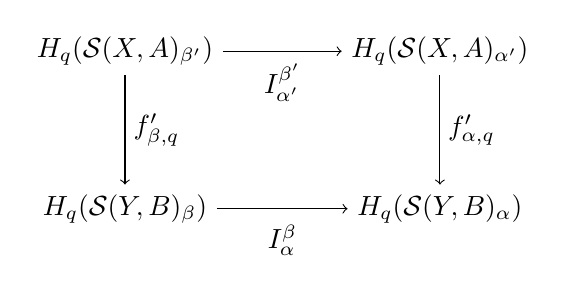
\begin{tikzpicture}
	
	
	
	\node (w) at (0,0) {\(H_q(\mathcal{S}(X,A)_{\beta'})\)};
	
	\node (x) at (0,-2) {\(H_q(\mathcal{S}(Y,B)_{\beta})\)};
	
	\node (y) at (4,-2) {\(H_q(\mathcal{S}(Y,B)_{\alpha})\)};
	
	\node (z) at (4,0) {\(H_q(\mathcal{S}(X,A)_{\alpha'})\)};
	
	\node (f) at (2,-2.4){\(I^\beta_\alpha\)};
	
	\node (g) at (2,-0.4){\(I^{\beta'}_{\alpha'}\)};
	
	\node (s) at (0.4,-1) {\(f'_{\beta,q}\)};
	
	\node (s2) at (4.4,-1) {\(f'_{\alpha,q}\)};	
	
	\draw[->] (z) -- (y);
	\draw[->] (w) -- (x);
	\draw[->] (x) -- (y);
	\draw[->] (w) -- (z);
	
	
	\end{tikzpicture}
	$$
	
The fact that collection $\mathcal{A}_q$ is natural transformation of the groups follows directly from the above diagram. Thus by lemma \ref{limitmorphismgroup} there exists limit homomorphism $$f_q:\check{\mathrm{H}}_q(X,A;G) \rightarrow \check{\mathrm{H}}_q(Y,B;G) $$
\end{proof}
We will show now that the Cech homology group is a functor. 
\begin{lause}
Cech homology groups are functors from the category of the topological pairs to the category of abelian groups 
\end{lause}
\begin{proof}
\begin{enumerate}[label=(\arabic*),ref=(\arabic*)]
\item Every pair of spaces is mapped uniquely to some abelian group.
\item The limit of identity map is an identity homomorphism.
\item Let $f:(X,A) \rightarrow (Y,B)$ and $g:(Y,B) \rightarrow (Z,C)$ be continuous maps between pairs. We know that $(g \circ f)_{*} = g_* \circ f_*$ holds for the singular homology groups. Then by using theorem \ref{compositionlimitmorphism} we see that the limit homomorphism $\lim ((g \circ f)_*)$ equals $\lim g_* \circ \lim f_*$.
\end{enumerate}
\end{proof}


\section{Dimension axiom}
In this section we will prove that the cech homology theory satisfies the dimension axiom.
\begin{lause}

\end{lause}

\chapter{Applications}

\section{Lefschetz fixed-point theorem}
[Theory of this will be presented later]

\section{Kakutani fixed point theorem}

The fixed point theorem of Kakutani can be derived for Lefchetz fixed-point theorem.

\begin{maar}
Let $X$ be vector space with topological structure and $K$ topological field. If vector addition $+:X \times X \rightarrow X$ and scalar multiplication $\cdot:K \times X \rightarrow X $ are continuous we say that $X$ is topological vector space over field $K$ or shortly $L(X,K)$ 
\end{maar}
Topological vector space has following property:
\begin{lause}
Kakutani fixed point theorem. Let $S$ be a non empty, compact and convex subset of a locally convex Hausdorff space. Let $f:S \rightarrow 2^s$ be a multivalued function on $S$ which has closed graph and the property that $f(x)$ is convex and non-empty for all $x \in S$. Then the set of fixed points of $f$ is non-empty and compact.
\end{lause}



\section{Continuous game theory}
In this section we will apply theory developed in previous chapters to game theory. We define $n$ player continuous game structure $Cgs(J, \mathcal{A})$ in a following way:

\begin{maar}
Let $J$ be finite indexing set and $\mathcal{A}$ collection of continuous utility functions $\{u_i:X_i \rightarrow \R \}_{i \in J}$ with a compact domain. Then we say that $Cgs(J, \mathcal{A})$ is a continuous game.
\end{maar}
Now we give definition of Nash equilibrium for Cgs.

\begin{maar}
Let $Cgs(J, \mathcal{A})$ be continuous game we say that point $x^{*} \in \prod_{i \in J}X_i$ is Nash equilibrium if for every $k \in J$ and every $x'_k \in X_k$ following condition holds:
$$u_k(x*) \geq u_k(x_1, ..., x'_k, ... , x_n) $$ 
\end{maar}
Next we will prove important lemma which says that game has equilibrium only and only if specific function has fixed point. 
\begin{lem}
$Cgs(n, \mathcal{A})$ has Nash equilibrium only and only if following set value function $$g:\prod_{i \in J}X_i \rightarrow \prod_{i \in J}2^{X_i}: g_k(x) = \argmax_{t \in X_k}u_k(x_1, ... x_{k}, t, x_{k+1},...,x_{n})$$
has a fixed point $x \in g(x)$  
\end{lem}
\begin{proof}
Trivial (Just check definitions)
\end{proof}

\subsection{General version of resource optimization problem}
Consider a game where a set of players compete in a multiple competitions at the same. Every player has limited energy and they can allocate it freely. Every competition is won by a player who allocated most energy in it and the goal of the players is to maximize the amount of the competitions they win.

\begin{maar}
We define the continuous game structure of the game described above as follows:
\begin{enumerate}
\item The choice space for every player consists of continuous functions $f:[0,1]\rightarrow \R$ for which $\int_{0}^{1}f(x) dx = 1 $
\item The evaluation function $u_n(x):\prod_{i \in J}X_i \rightarrow [0,1]$ is defined to be: $$u_n(f) = m^*(\{x \in [0,1] \mid f_n(x) \geq f_i(x)\})$$
\end{enumerate}
\end{maar}
We will show that in some cases there exists an equalibrium.


\begin{thebibliography}{9}
\item

\bibitem{Rotman}\label{rotman}

J. Rotman An Introduction to Algebraic Topology (Graduate Texts in Mathematics), Springer 

\bibitem{First}
L. G�rniewicz, Topological Fixed Point Theory of Multivalued Mappings, Kluwer Academic
Publishers, 1999.

\bibitem{Second} 
I. L. Glicksberg, A further generalization of the Kakutani fixed point theorem with
application to Nash equilibrium points, Proc. Amer. Math. Soc. 3 (1952), 170�174.


\bibitem{Vaisala}\label{vai}
M. BAYE, G. TIAN, ANU J. ZHOU, �The Existence of Pure Nash Equilibrium in Games 
with Nonquasiconcave Payoffs,� Texas A  M University, mimeo, 1990. 

\bibitem{categorytheory}\label{categorytheory}
Saunders Mac Lane: Categories for the Working Mathematician (Graduate Texts in Mathematics)

\bibitem{algebra2}\label{algebra2}
Jokke H�s�: Algebra II, 2016. 

\end{thebibliography}

\end{document}
